\documentclass[12pt]{article}
\usepackage{tikz}
\usepackage{pgf-umlcd}
\usepackage{amsmath}
\usepackage{amsfonts}
\usepackage{pdflscape}
\usepackage{fancyhdr}
\usepackage{ulem}
\usepackage{graphicx}
\usepackage{bold-extra}
\usepackage[colorlinks = true,
            linkcolor = magenta,
            urlcolor = magenta,
            citecolor = magenta,
            anchorcolor = magenta]{hyperref}
\usepackage{url}
\usepackage[top = .75in, left = .75in, right = .75in, bottom = 1in]{geometry}

% Table
\usepackage{array}

% For algorithm
\usepackage{algorithm}
\usepackage{algpseudocode}

% For code
\usepackage{listings}
\usepackage{xcolor}
\definecolor{codegreen}{rgb}{0, 0.6, 0}
\definecolor{codegray}{rgb}{0.5, 0.5, 0.5}
\definecolor{codepurple}{rgb}{0.58, 0, 0.82}
\definecolor{backcolour}{rgb}{0.95, 0.95, 0.92}

\lstdefinestyle{mystyle} {
    backgroundcolor = \color{backcolour},
    commentstyle = \color{codegreen},
    keywordstyle = \color{magenta},
    numberstyle = \tiny\color{codegray},
    stringstyle = \color{codepurple},
    basicstyle = \ttfamily\footnotesize,
    breakatwhitespace = false,
    breaklines = true,
    captionpos = b,
    keepspaces = true,
    numbers = left,
    numbersep = 5pt,
    showspaces = false,
    showstringspaces = false,
    showtabs = false,
    tabsize = 2
}
\lstset{style = mystyle}

\setlength{\parindent}{0pt}

\newcommand{\coursename}{Fundamentals of Programming}
\newcommand{\reportname}{Final Project}
\newcommand{\reporttitle}{Poker Game}

\newcommand{\studentname}{Lam Chi Hao \\ Vo Nhat Tien \\ Le Nguyen Anh Tri}
\newcommand{\teachername}{Nguyen Hai Minh \\ Tran Thi Thao Nhi \\ Phan Thi Phuong Uyen}


% ============ HEADER AND FOOTER ============
% Header length
\setlength{\headheight}{29.43912pt}

% Footer page number would be on the lower-right corner
\pagestyle{fancy}
\fancyfoot{}
\fancyfoot[R]{Page \thepage}

\lhead{\reporttitle}
\rhead{\coursename}

%\lfoot{\leftfooter}
\renewcommand{\footrulewidth}{0.4pt}
\lfoot{University of Science - VNU-HCM}

% Footer page number for landscape
\fancypagestyle{lscape}{
\fancyhf{}
\fancyfoot[R]{Page\thepage}
\renewcommand{\headrulewidth}{0pt} 
\renewcommand{\footrulewidth}{0pt}
}

%Document
\begin{document}

% Cover paper
\begin{titlepage}
    \newcommand{\HRule}{\rule{\linewidth}{0.5mm}}
    \centering
    
    \textsc{\LARGE viet nam national university ho chi minh city}\\ [0.5cm]
    \textsc{\large university of science} \\ [0.5cm]
    \textsc{\large faculty of information technology} \\ [0.5cm]
    
    \includegraphics[scale = 0.36]{figures/hcmus-logo.jpeg} \\ [0cm]
    \HRule \\ [0.2cm]
    {
    \huge{\bfseries{\reporttitle}}\\[0.2cm]
    \Large{\bfseries{Report Name: \reportname}}
    }
    \\[0.2cm]
    \HRule \\ [0.2cm]
    
    \textbf{\large Course name: \coursename}\\ [0.3cm]
    \textbf{\large CSC1002 - 24C03} \\ [1.3cm]
    
    \begin{minipage}[t]{0.4\textwidth}
    \begin{flushleft} \large
    \emph{Student name: }\\
    \studentname
    \end{flushleft}
    \end{minipage}
    ~
    \begin{minipage}[t]{0.4\textwidth}
    \begin{flushright} \Large
    \emph{Teacher name: } \\
    \teachername
    \end{flushright}
    \end{minipage} \\[4.2cm]
    {\large 07/12/2024} \\[0.4cm]
    \vfill
    
\end{titlepage}

% ------------------- THE END ------------------- %

\tableofcontents
\pagebreak

% Introduction
\section{Foreword}
\label{sec:foreword}

\hspace{1cm} We would like to give our most sincere thanks to Mrs. Tran Thi Thao Nhi and Mrs. Phan Thi Phuong Uyen for this opportunity to do the project. Your valuable advice and encouragement during the course of our work mean a great deal to us, and we cannot appreciate enough the time and effort you have devoted to making us successful. We hope that our results satisfy your expectations.

\vspace{0.5cm}

\hspace{1cm} Although the project is not without its limitations, such as one of our team members being unable to contribute due to his personal circumstances, we have done our best to complete it. We would appreciate your understanding of our situation and the effort we have put into overcoming these challenges.

\vspace{0.5cm}

\hspace{1cm} We really do hope you will like the project and that it lives up to your vision. Your valued comments and feedback will go a long way in our growth and service improvement in the future.

\vspace{0.5cm}

\hspace{1cm} We are particularly very lucky to have been in this project for experience and learning. Any shortcomings and mistakes are solely our own liability, and we take this as an opportunity to improve our skill and knowledge further.

\vspace{0.5cm}

\hspace{1cm} Thank you once more for sparing your valuable time and considering our request. It was an honor and a pleasure working under your guidance, and we hope that someday in life, we get to work with you again.

\vspace{0.5cm}

\hspace{1cm} Best regards,

% ------------------- THE END ------------------- %

\pagebreak
\section{Introduction}
\label{sec:introduction}

% GROUP INFORMATION
\hspace{1cm} This project focused on developing a Poker game using the C++11 programming language. It was done in a group of two members, Le Nguyen Anh Tri and Lam Chi Hao (originally three members, but Vo Nhat Tien was unable to contribute due to personal circumstances), for the final project of the course Fundamentals of Programming (CSC10012) at the University of Science, Vietnam National University — Ho Chi Minh City.

\vspace{0.5cm}

\hspace{1cm} Here is our group information for this project:

\begin{table}[ht]
    \centering
    \begin{tabular}{| m{1.75cm} | m{2cm} | m{5cm}| m{2.5cm} |} 
    \hline
    \textbf{} & \textbf{ID} & \textbf{Name} & \textbf{Title} \\ 
    \hline
    1 & 24127034 & Lam Chi Hao & Leader \\ 
    \hline
    2 & 24127567 & Le Nguyen Anh Tri & Member \\ 
    \hline
    \end{tabular}
    \caption{Information of Group 02 member.}
    \label{tab:group-information}
\end{table}

\hspace{1cm} Group management and communication were pretty simple in our two-man team. Messenger served us for fast discussions, while GitHub was used for versioning and collaboration. This simplicity excluded any formal work management board or a developed communication plan. So, roles were divided quite clearly: one team member worked on core game logic, while the second was developing a GUI. Then we will take our time to review the code, test, and make merges towards the end that would bring everything together as needed.

\vspace{0.5cm}

\hspace{1cm} This is our table of contributions for this project, which shows the work we have done.

\begin{table}[ht]
    \centering
    \begin{tabular}{|m{4cm}|m{2cm}|m{2cm}|m{2cm}| m{2cm}|}
    \hline
    \textbf{Problem} & \textbf{Rubric} & \textbf{24127034} & \textbf{24127557} & \textbf{24127567} \\
    \hline
    Standard features & - &  &  &  \\
    \hline
    Initialization & 20 & 5 & 0 & 15 \\
    \hline
    Dealing & 20 & 0 & 0 & 20 \\
    \hline 
    Gameplay & 20 & 0 & 0 & 20 \\
    \hline
    Player's information & 20 & 5 & 0 & 15 \\
    \hline
    Advanced features & - &  &  &  \\
    \hline 
    Draw poker & 30 & 15 & 0 & 15 \\
    \hline
    5-card stud & 30 & 0 & 0 & 0 \\
    \hline
    Color / Sound effects & 30 & 30 & 0 & 0 \\
    \hline
    Leader board & 30 & 10 & 0 & 20 \\
    \hline
    Hash password & 10 & 0 & 0 & 10 \\
    \hline
    Makefile & 10 & 5 & 0 & 5 \\
    \hline
    % Creations & 30 / each & Score & Score & Score \\
    % \hline
    Report & - &  &  &  \\
    \hline
     & 100 & 70 & 0 & 30 \\
    \hline
    & Total & 135 & 0 & 140 \\
    \hline
    \end{tabular}
    \caption{Table of contribution}
    \label{tab:contribution-table}
\end{table}

\hspace{1cm} This project breaks into three significant parts, which are the core game logic, the GUI, and the testing process, which make up the majority of the work. The core game logic was the most challenging part, as it required a deep understanding of the game rules and the ability to implement them in C++. The GUI was the most time-consuming part, as it required a lot of trial and error to get the layout and design right. The testing process was the most tedious part, as it required a lot of manual testing to ensure that the game was bug-free and worked as expected. Each part of the project had its challenges, but we were able to overcome them by working together and supporting each other throughout the process, more details will be discussed in each of the following sections.

\vspace{0.5cm}

\hspace{1cm} To enhance the project a little further, we used the SDL2 library to create a graphical user interface for the Poker game. Such a GUI makes interactions with the game much easier and fun. It gives good visual clarity so that one understands the actual happening of the game better. In that way, by integrating SDL2 into our project, we made it more fun, not to mention challenging, as well.

\subsection{About the Poker Game}
\label{subsec:about-the-poker-game}

\subsubsection{Poker Hand Rakings}
\label{subsubsec:poker-hand-rankings}
\hspace{1cm} In Poker, a hand comprises five cards, regardless of whether the cards are from a single deck or different decks, provided the number is five altogether. Below are the official poker hand rankings, in order from highest to lowest.

\begin{enumerate}
    \item \textbf{Royal Flush}: The best possible poker hand, formed by the Ace, King, Queen, Jack, and 10, all of the same suit, for example, hearts. (Note: This hand is not implemented in our project since it is very rare and not called for in the project specification.)
    \item \textbf{Straight Flush}: Five sequential cards all of one suit (such as 9, 8, 7, 6, 5, all hearts).
    \item \textbf{Four of a Kind}: Four cards of one rank (such as four Aces).
    \item \textbf{Full House}: Three cards of one rank and two cards of another rank (such as three Kings and two 4s).
    \item \textbf{Flush}: Any five cards of the same suit, but not in sequential order (such as 2, 4, 6, 9, King, all in diamonds).
    \item \textbf{Straight}: Five consecutive cards of different suits, like 10 of hearts, Jack of spades, Queen of diamonds, King of clubs, Ace of hearts.
    \item \textbf{Three of a Kind}: Three cards of the same rank, such as three 7s.
    \item \textbf{Two Pair}: Two cards of one rank and two cards of another rank, such as two 5s and two 9s.
    \item \textbf{One Pair}: Two cards of the same rank, such as two 8s.
    \item \textbf{High Card}: If no other hand is made, then the highest card played becomes the rank (such as King, 10, 8, 6, 4; this would be a "King-high" hand).
\end{enumerate}

\hspace{1cm} In all, there are 10 possible poker hands that range from the highest, Royal Flush, to the lowest, High Card. However, in this project, we will implement only hands ranked from Straight Flush to High Card due to the requirements of our project, since it is too rare to happen and the project requirements do not include this as well.

\subsubsection{Poker Game Variants}
\label{subsubsec:poker-game-variants}

\hspace{1cm} Based on that information, there are a lot of variants of Poker, and each has its own rules and way of playing. Some popular variants includes:

\begin{enumerate}
    \item \textbf{Texas Hold'em}: Each player is dealt two private cards, and then five community cards are turned over on the table; players can use any number of these seven cards in attempting to build the highest possible five-card hand.
    \item \textbf{Draw Poker}: Players are dealt five cards and can choose to discard and replace some of them (typically 1 to 3 cards at a time). After this, the player with the best hand wins. The gameplay is structured as follows:
    \begin{itemize}
        \item \textbf{Round 1}: All players are dealt 5 cards each. Players must now decide whether to play by selecting "raise", "call" or "fold".
        \item \textbf{Round 2}: Players can discard and replace one to three cards once (in some versions, if a player has an Ace, he/she can discard four cards and draw four new ones).
        \item \textbf{Round 3}: Players decide again to either "raise", "call", or "fold" depending on their now improved hands.
        \item \textbf{Round 4}: Hands are revealed, and the player with the highest hand wins.
    \end{itemize}
    \item \textbf{Stud Poker}: Some cards are dealt face up and others face down, with several rounds of betting. The highest five-card hand wins the game.
    \item \textbf{Simplified Poker}: This is a Poker variant, included in the project requirements, and is subject to the rules listed below: Each player is initially dealt 5 cards. The player with the highest-ranking hand wins. In case of a tie, when two players hold the same hand, it is won by the player with the highest-ranking card. If two or more players have the same hand and the same high card, then the pot is divided equally.
\end{enumerate}

\hspace{1cm} We are going to implement two game variants: Simplified Poker and Draw Poker. Even though the Simplified Poker game fulfilled all the basic requirements set in the project, we felt it was a bit simple and basic. In order to make the project exciting and challenging, we decided to implement the Draw Poker variant. This is an extension of the framework set by the Simplified Poker game, further allowing us to fulfill some of the advanced requirements stipulated in the project.

\subsection{Class structure of the Poker Game}
\label{subsec:class-structure-of-the-poker-game}

\hspace{1cm} In this project, we have deliberately avoided creating separate, isolated codebases for each game mode that we would like to have. Instead, we designed a unified structure, which contains all game modes under one implementation. This will let us take advantage of the object-oriented features of C++ - that is classes introduced in C++11—to achieve modularity and expandability. By doing so, we can easily modify or extend the project with more game modes in the future without rewriting the whole codebase.


\subsubsection{Class Design}
\label{subsubsec:class-design}

\hspace{1cm} The game of Poker was implemented by using the C++ programming language with SDL2 library and IDE Visual Studio Code. For this, we used the C++11 class feature to design and implement the game. In fact, this usage of classes is beyond the basic requirements of the project. We did it for the following two main reasons:

\begin{enumerate}
    \item \textbf{Pratical Learning}: This exercise used classes, which is good programming practice and prepares us for future, more complex projects.
    \item \textbf{Efficiency}: Classes allow for encapsulation of data and methods, making it easier to extend functionality and organize compared to the traditional struct in C99.
\end{enumerate}

\hspace{1cm} In this project, we used classes in a way similar to how \texttt{struct} would be used in C99, with the added flexibility - thanks to encapsulation - of being able to pack both data and behavior. This allowed us to create better organized code that is maintainable and more readable.

\vspace{0.5cm}

\hspace{1cm} The classes we used in this project are as follows. (About the details, we will explain each of the classes we have implemented for this project in the \hyperref[sec:implementation-of-the-poker-game]{Implementation} section).
\begin{enumerate}
    \item \textbf{\texttt{Card}}: This class represents a single card in the deck. It contains two private members: \texttt{enum Ranks} and \texttt{enum Suits}. The class also contains some public methods for debug purpose that returns the card in the form of a string.
    \item \textbf{\texttt{Deck}}: This class represents a standard 52-card deck. This class has methods for handling things like shuffling, dealing, and resetting the deck.
    \item \textbf{\texttt{Strength}}: This class represents the strength of a hand in Poker based on what we've discussed in the \hyperref[subsubsec:poker-hand-rankings]{Poker Hand Rankings}, which containing methods to evaluate and compare hands.
    \item \textbf{\texttt{Hand}}: This class represents a hand of cards in the game, help us handling things like sorting and evaluating the hand of players.
    \item \textbf{\texttt{Storage}}: Represent a storage that stores player information, handling reading and writing player data to a file.
    \item \textbf{\texttt{Leaderboard}}: Represents the leaderboard, handling reading and writing leaderboard data to a file.
    \item \textbf{\texttt{Player}}: Contains all necessary player information used in the game. This class encapsulate various attributes associated with the players. It includes public memeber variables such as \texttt{string username}, \texttt{float chips}, \texttt{unsigned int winningStrategy[9]} (since there are 9 combinations of Poker hand being covered in this project), and so on.
    \item \textbf{\texttt{Gameplay}}: This class encapsulates the core components such as the deck of cards via \texttt{Deck} and player data via \texttt{Player}. It provides methods to initialize the game with players and bots, deal cards, manage player actions, determine the winner, and maintain a leaderboard. By centralizing these functionalities, the \texttt{Gameplay} class ensures that the game logic is organized, making the codebase easier to maintain and extend. This class is essential for coordinating the various elements of the game, ensuring a smooth and coherent gameplay experience.
    \item \textbf{\texttt{Lobby}}: This class manages the players and bots waiting for a game to start. It provides methods to add and remove players via username and handle the number of players in the lobby. By keeping track of the players and bots in the lobby, the \texttt{Lobby} class ensures that the game can start with the correct number of players.
    \item \textbf{\texttt{GameEngine}}: This is the core component of the entire game application, responsible for managing the main game loop and handling the game states and events. It manages things related to initialization, event handling, updating, rendering, and the cleanup processes. This class ensure the game run correctly, make things easier to scale up and maintain.
\end{enumerate}

\subsubsection{Class Diagram}
\label{subsubsec:class-diagram}
\hspace{1cm} The following diagram illustrates the main classes and their relationships in the poker game:

\begin{figure}[H]
    \centering
    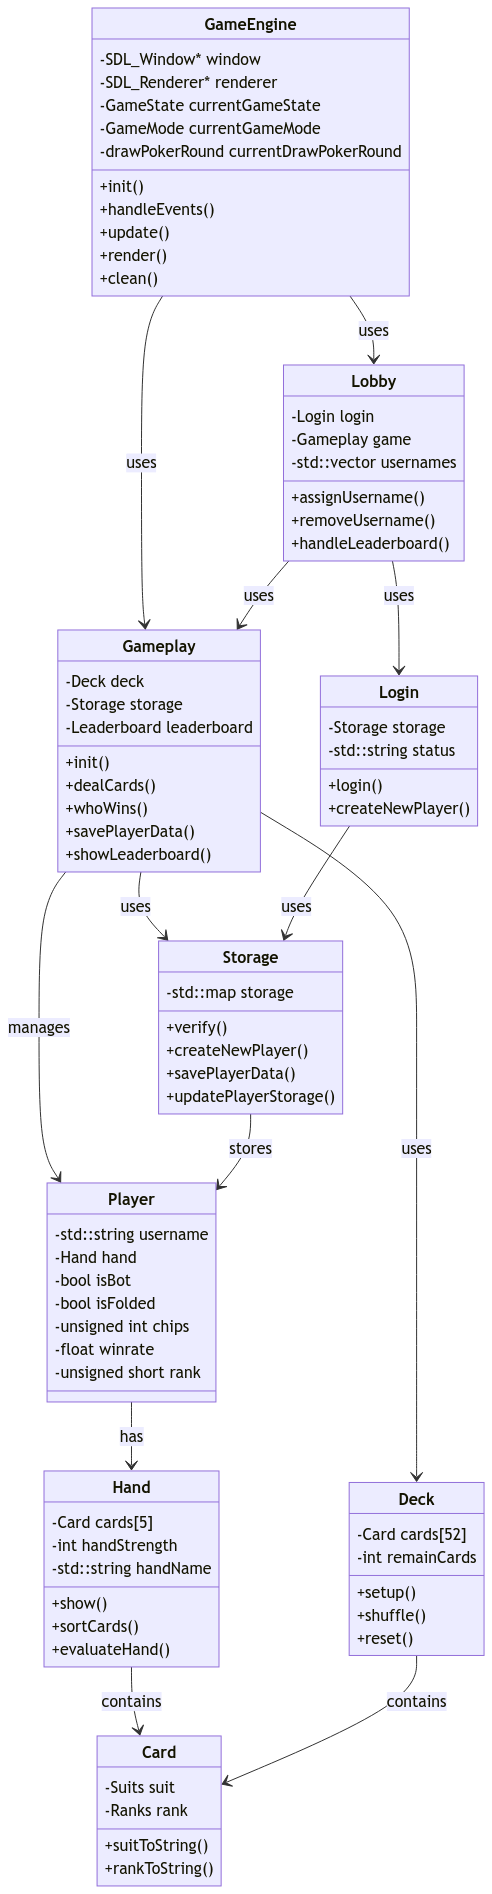
\includegraphics[width=125pt]{figures/class-diagram.png}
    \caption{Class Diagram of the Poker Game}
    \label{fig:class-diagram}
\end{figure}

\subsection{Naming Convention of the Project}
\label{subsec:naming-convention-of the-project}

\hspace{1cm} For this part of the report, we will discuss the project structure, including the folder structure, file structure, variable, constant, class, as well as struct naming conventions.

\vspace{0.5cm}

\hspace{1cm} The naming convention is a set of rules for choosing the character sequence to represent the name of a variable, constant, function, class, file, folder, or other entity in the source code. The naming convention is essential because it helps the reader understand the code more easily and quickly. In this project, we follow the naming convention below:

\subsubsection{Folder}
\label{subsubsec:folder}

\hspace{1cm} We decide that all folder names are named in lowercase and separated by an underscore. There are two main rules for naming folders in our project:

\begin{itemize}
    \item \textbf{lowercase}: All characters in the folder name are lowercase.
    \item \textbf{Underscore}: If the folder name consists of multiple words, separate them with an underscore.
\end{itemize}

\subsubsection{File}
\label{subsubsec:file}

\hspace{1cm} We decide that all file names are named in lowercase and separated by an underscore or hyphen. There are three main rules for naming files in our project:

\begin{itemize}
    \item \textbf{lowercase}: Only one exception is our main file, which is named \textbf{main.cpp}.
    \item \textbf{CamelCase}: We decide that all of the header files and source files are named in CamelCase.
    \item \textbf{Underscore \& hyphen}: This is for files in SDL2 libraries, which are named in lowercase and separated by an underscore. Besides that, our files in assets are named in lowercase and separated by an underscore or hyphen.
\end{itemize}

\subsubsection{Variable, constant, class, struct}
\label{subsubsec:variable-constant-class-struct}

\hspace{1cm} We decide that all of the variables, constants, classes, and structures are named in camelCase, CamelCase, and ALL\_CAPS. There are three main rules for naming variables, constants, classes, and structures in our project:

\begin{itemize}
    \item \textbf{camelCase}: We decide that all of the variables are named in camelCase. Notice that the first letter of the first word is lowercase, and the first letter of the following words is uppercase.
    \item \textbf{CamelCase}: For classes and structures in our project, we decide that all of the classes and structures are named in CamelCase. Notice that the first letter of each word is uppercase.
    \item \textbf{ALL\_CAPS}: We decide that all of the constants are named in ALL CAPS. Notice that if the constant consists of multiple words, we will separate them with an underscore.
\end{itemize}

\subsubsection{Function Prototype and Definition}
\label{subsubsec:function-prototype-definition}

\hspace{1cm} We decide that all of the functions are named in camelCase. Notice that the first letter of the first word is lowercase, and the first letter of the following words is uppercase.

\subsection{Folder structure of the Project}
\label{subsec:folder-structure-of-the-project}

\hspace{1cm} After discussing, we decided that the project structure will be organized as follows. This structure ensures that the project is well-organized, making it easier to navigate, maintain, and scale. Each folder and file has a specific purpose, and the naming conventions are designed to be intuitive and consistent. Below is a detailed breakdown of the project structure:

\begin{itemize}
    \item \textbf{src}: Contains all source code files written in C++. There are two subfolders with two main categories of source code files.
    \begin{itemize}
        \item \textbf{core}: Contains all the source files related to the core mechanics of the game.
        \item \textbf{gui}: Contains all the source files related to the graphical user interface of the game.
    \end{itemize}
    \item \textbf{include}: Contains all header files. There are two subfolders with two main categories of header files.
    \begin{itemize}
        \item \textbf{core}: Contains all the header files related to the core mechanics of the game.
        \item \textbf{gui}: Contains all the header files related to the graphical user interface of the game.
    \end{itemize}
    \item \textbf{bin}: Contains all executable files, object files, and dynamic libraries. There is a subfolder called obj. Inside the obj folder, there are two subfolders with two main categories of object files.
    \begin{itemize}
        \item \textbf{core}: Contains all the object files related to the core mechanics of the game.
        \item \textbf{gui}: Contains all the object files related to the graphical user interface of the game.
    \end{itemize}
    \item \textbf{assets}: Contains all assets used in the project. There are three subfolders inside our assets folder.
    \begin{itemize}
        \item \textbf{imgs}: Contains all images used in the project. There are images for backgrounds, buttons, cards, cursor, and icons for our game application.
        \item \textbf{audios}: Contains all sounds used in the project. There are audios for background music, button click sound, card shuffle sound, and card flip sound.
        \item \textbf{fonts}: Contains all fonts used in the project. There are fonts for the game title, game buttons, and game text.
    \end{itemize}
    \item \textbf{libs}: Contains all libraries used in the project.
    \begin{itemize}
        \item \textbf{SDL2}: Contains all SDL2 libraries. This is our main library for creating the graphical user interface.
        \item \textbf{cmake}: Contains all CMake libraries.
    \end{itemize}
    \item \textbf{report}: Contains all report files which are source code files written in LaTeX.
    \begin{itemize}
        \item \textbf{contents}: Contains all the contents of the report. We want to keep the report organized, so we separate the report into multiple files and put them in the contents folder.
        \item \textbf{figures}: Contains all figures used in the report. The figures are images, graphs, tables, etc.
    \end{itemize}
\end{itemize}

% ------------------- THE END ------------------- %
\pagebreak
\section{Implementation of the Poker Game}
\label{sec:implementation-of-the-poker-game}

\subsection{Included Library}
\label{subsec:included-library}

\hspace{1cm} For this project to work, we need to include some libraries, and step on that to build the project. These libraries are from the standard library of C++ and we use them to implement the project. The libraries that we include in this project are:
\begin{enumerate}
    \item \textbf{\texttt{<iostream>}}: In this project, we used to handle most of our debug statements on the console while running and developing the project. This library is used to handle the input and output stream.
    \item \textbf{\texttt{<string>}}: This library is used to handle string data types. We use this library to handle the name of the player, the password of the player, the name of the game, and so on. The string is also used to handle the input and output login, register, and render text process.
    \item \textbf{\texttt{<vector>}}: This library is used to handle the dynamic array. Some of the data that we need to handle in the dynamic array are the \texttt{strengthCards} since those cards that form the hand of the player are dynamic, (we don't know how many cards the player will have to form a hand at compile time).
    \item \textbf{\texttt{<map>}}: This library is used to handle the key-value pair. Especially in the \texttt{Storage} class, we use this library to handle the key-value pair of the player's data and their username as a key.
    \item \textbf{\texttt{<random>}}: In this project, we use \texttt{random} to generate random numbers. We use this library as a helper to shuffle the deck of cards.
    \item \textbf{\texttt{<algorithm>}}: This library is used to handle the algorithm. We use this library to handle the sorting of the cards in the player's hand. We configured the basic sorting algorithm to sort the cards in the player's hand by their rank.
    \item \textbf{\texttt{<ctime>}}: This library is used to handle the time. We use this library to handle the seed of the random number generator. We use the current time as the seed of the random number generator.
    \item \textbf{\texttt{<funtional>}}: This library is used to handle the function object. We use this library to handle the comparison of the cards in the player's hand. We configured the basic comparison function object to compare the cards in the player's hand by their rank. This provides us will the ability to create a lambda function for a custom comparison function.
    \item \textbf{\texttt{<fstream>}}: This library is used to handle the file stream. Especially in the \texttt{Storage} class, we use this library to handle the file stream of the player data and the leaderboard data. We use this library for reading, writing, and appending the data to the file.
    \item \textbf{\texttt{<sstream>}}: This library is used to handle the string stream. Especially in the \texttt{Storage} class, we use this library to handle the parsing of the player's data and the leaderboard data.
\end{enumerate}

\hspace{1cm} Beside the standard library of C++11, we also include the SDL2 library to handle the graphical user interface of the project. The libraries that we include in this project are:
\begin{enumerate}
    \item \textbf{\texttt{<SDL2/SDL.h>}}: This library is used to handle the basic SDL2 library. We use this library to handle the basic initialization of the SDL2 library.
    \item \textbf{\texttt{<SDL2/SDL\_image.h>}}: This library is used to handle the image library of the SDL2. We use this library to handle the image loading and rendering process.
    \item \textbf{\texttt{<SDL2/SDL\_ttf.h>}}: This library is used to handle the True Type Font library of the SDL2. We use this library to handle the text rendering process.
    \item \textbf{\texttt{<SDL2/SDL\_mixer.h>}}: This library is used to handle the audio library of the SDL2. We use this library to handle the audio loading and playing process.
\end{enumerate}

\hspace{1cm} Notice that we don't include the \texttt{<SDL2/SDL\_net.h>} library in this project. This is because we do not use the network library of SDL2 in this project. We only use the basic SDL2 library, image library, True Type Font library, and audio library.

\subsection{Precompiled Header}
\label{subsec:precompiled-header}

\hspace{1cm} In order to speed up the compilation process, we decided to use the precompiled header in our project. The precompiled header is a header file that is compiled into a binary file that can be used by the compiler to speed up the compilation process. The precompiled header is used to store the header files that are frequently used in the project. By using the precompiled header, the compiler doesn't need to recompile the header files that are stored in the precompiled header. This will speed up the compilation process since the compiler doesn't need to recompile the header files that are stored in the precompiled header.

\vspace{0.5cm}

\hspace{1cm} To implement that, we create a header file called \texttt{pch.h} and include all the necessary header files, especially frequent and heavy-weighted header files such as SDL2 libraries. We include the \texttt{pch.h} in every source file for the graphical user interface. Then we compile the \texttt{pch.h} into a binary file called \texttt{pch.pch}. This will speed up the compilation process since the compiler doesn't need to recompile the header files. Otherwise, the compiler will need to compile every time for every source file that includes the SDL2 libraries. \href{https://github.com/anhtri2407/Poker/blob/main/include/pch.h}{Precompiled header source code}.

\vspace{0.5cm}

\hspace{1cm} Also in that precompiled header file, we define lots of our (constexpr) constants that are used to determine the path of our game assets such as images, fonts, and audio at compile time. This will make the code more readable and maintainable since we don't need to hardcode the path of the game assets in every source file. We only need to include the precompiled header file and use the constants that are defined in the precompiled header file.

\subsection{Makefile}
\label{subsec:makefile}

\hspace{1cm} In this project, we use a Makefile to manage the build process. A \texttt{Makefile} is a simple way to define a set of tasks to be executed. It is commonly used to compile and build programs. The Makefile contains rules that specify how to compile and link the program. Each rule consists of a target, dependencies, and commands. The Makefile is processed by the make utility, which executes the commands to build the target.

\vspace{0.5cm}

\hspace{1cm} Since this project is relatively small and simple, we decided to use a Makefile to manage the build process. The Makefile is straightforward and easy to understand, making it suitable for this project. 
\vspace{0.5cm}

\hspace{1cm} To implement that we create a file called \texttt{Makefile}, which is a simple text file that contains a list of commands to be executed by the make command. These commands are used to compile the project, link the libraries, and generate the executable file. \href{https://github.com/anhtri2407/Poker/blob/main/Makefile}{Makefile source code}.

\vspace{0.5cm}

\hspace{1cm} Notice that we've just implemented the \texttt{Makefile} for just Windows and MacOS, some of the Unix-based operating systems. We haven't implemented the \texttt{Makefile} for Linux yet. Since we don't have a Linux operating system computer to test the \texttt{Makefile} implementation. So, we can't guarantee that the \texttt{Makefile} implementation will work on Linux.

\vspace{0.5cm}

\hspace{1cm} To run the \texttt{Makefile}, we need to open the terminal and navigate to the root directory of the project. Then we run the following steps: (Note: you can read more about these steps in our \href{https://github.com/anhtri2407/Poker/blob/main/README.md}{README.md} file.
\begin{enumerate}
    \item \textbf{\texttt{make clean}}: This command is used to clean the project. It will remove all the object files and the executable file.
    \item \textbf{\texttt{make all}}: This command is used to compile the project. It will compile the source files, link the libraries, and generate the executable file.
    \item \textbf{\texttt{make run}}: This command is used to run the project. It will run the executable file.
\end{enumerate}

\hspace{1cm} On Windows operating system, we need to install the \texttt{mingw-w64} compiler to run the \texttt{Makefile}. We also need to add the \texttt{mingw-w64} compiler to the system environment variable. This will allow us to run the \texttt{Makefile} on the Windows operating system by the following steps:
\begin{enumerate}
    \item \textbf{\texttt{mingw32-make -f Makefile clean}}: This command is used to clean the project. It will remove all the object files and the executable file.
    \item \textbf{\texttt{mingw32-make -f Makefile all}}: This command is used to compile the project. It will compile the source files, link the libraries, and generate the executable file.
    \item \textbf{\texttt{mingw32-make -f Makefile run}}: This command is used to run the project. It will run the executable file.
\end{enumerate}

\subsection{Game Core}
\label{subsec:game-core}
\begin{enumerate}
    \item \textbf{Card}: This class is used to represent a single card in a standard 52-card deck. This class is used to define the suit and rank of a card. The suit and rank are represented by two enumerations, \texttt{Suits} and \texttt{Ranks}, respectively. The enumerate variable is initialized with the values of \texttt{-1} to \texttt{12} for the ranks and \texttt{-1} to \texttt{3} for the suits. The class also contains a method for printing the card to the console at the early state of the project. \href{https://github.com/anhtri2407/Poker/blob/main/src/core/Card.cpp}{Card Implementation}.
    \begin{itemize}
        \item \texttt{\textbf{suitToString()}}: string \\ This method converts the suit of the card to a string representation via a switch statement.
        \item \texttt{\textbf{rankToString()}}: string \\ This method converts the rank of the card to a string representation via a switch statement.
    \end{itemize}

    \item \textbf{Deck}: This class is used to represent a Standard 52-card deck. This class is built up using the \texttt{Card} class. The main idea is having an array of 52 objects of the type \texttt{Card} (Card cards[52]). In this file, we develop the methods for shuffling the deck, dealing with a card, and resetting the deck. \href{https://github.com/anhtri2407/Poker/blob/main/src/core/Deck.cpp}{Deck Implementation}.
    \begin{itemize}
        \item \texttt{\textbf{setup()}}: void \\ This method initializes the deck with 52 cards, one of each rank and suit.
        \item \texttt{\textbf{shuffle()}}: void \\ This method uses the \texttt{std::shuffle} function with a Mersenne Twister random number generator (\texttt{std::mt19937}) seeded with the current time (\texttt{std::time(0)}) to ensure a unique shuffle each time.
        \item \texttt{\textbf{reset()}}: void \\ This method simply calls the \texttt{setup()} method and then the \texttt{shuffle()} method to reset the deck. Also, set the remaining card back to 52.
    \end{itemize}

    \item \textbf{Strength}: This class is for represents the strength of a hand in Poker. This class contains methods for calculating the strength of a hand, and checking the rank of the hand as we've mentioned above \hyperref[subsubsec:poker-hand-rankings]{Poker Hand Rankings}.
    \begin{itemize}
        \item \texttt{\textbf{isStraightFlush(Hand)}}: bool \\ The idea is to loop through the first four cards in the sorted hand and check if each card has the same suit as the next card. If not, it will return \texttt{false}. If one pair of card's ranks are not consecutive, it will return \texttt{false}. If all the cards are consecutive and have the same suit, it will return \texttt{true}. Then assign these cards to \texttt{vector strengthCards}.
        \item \texttt{\textbf{isFourOfAKind(Hand)}}: bool \\ The idea is to check if the first four cards in the sorted hand have the same rank or if the last four cards in the sorted hand have the same rank. If so, it will return \texttt{true} and assign these four cards to \texttt{vector strengthCards}. Otherwise, it will return \texttt{false}.
        \item \texttt{\textbf{isFullHouse(Hand)}}: bool \\ The idea is to check if the first three cards and the last two cards in the \texttt{sortedCards[5]} have the same rank or the first two cards and the last three cards in the \texttt{sortedCards[5]} have the same rank. If so, it will return \texttt{true} and assign these five cards to \texttt{vector strengthCards}. Otherwise, it will return \texttt{false}.
        \item \texttt{\textbf{isFlush(Hand)}}: bool \\ The idea is to check if all five cards in the \texttt{sortedCards[5]} have the same suit by comparing the suit of each card to the next one. If all cards have the same suit, then it will return \texttt{true} and assign these five cards to \texttt{vector strengthCards}. Otherwise, it will return \texttt{false}.
        \item \texttt{\textbf{isStraight(Hand)}}: bool \\ The idea is using a loop to check if the first four cards in the \texttt{sortedCards[5]} have exactly one rank difference between the next card in the array. If all cards match that pattern, it will return \texttt{true} and assign these five cards to \texttt{vector strengthCards}. Otherwise, it will just return \texttt{false}.
        \item \texttt{\textbf{isThreeOfAKind(Hand)}}: bool \\ The idea is to check if all three possible consecutive combinations of three cards in the \texttt{sortedCards[5]} have the same rank. If any of these combinations match the pattern, then it will return \texttt{true} and assign these three cards to \texttt{vector strengthCards}. Otherwise, it will return \texttt{false}.
        \item \texttt{\textbf{isTwoPair(Hand)}}: bool \\ Since we have the sorted hand, the idea is to check if the first two cards and the next two cards in the \texttt{sortedCards[5]} have the same rank. Or the first two cards and the last two cards in the \texttt{sortedCards[5]} have the same rank. Or the second and the third cards and the last two cards in the \texttt{sortedCards[5]} have the same rank. If any of these conditions are met, it will return \texttt{true} and assign these four cards to \texttt{vector strengthCards}. Otherwise, it will return \texttt{false}.
        \item \texttt{\textbf{isOnePair(Hand)}}: bool \\ The idea is to check each consecutive pair of the cards in the \texttt{sortedCards[5]} from the first to the fourth card if they have the same rank or not. If any of these pairs have the same rank, it will return \texttt{true} and assign these two cards to \texttt{vector strengthCards}. Otherwise, it will return \texttt{false}.
        \item \texttt{\textbf{evaluateHand(Hand)}}: int \\ The idea behind this method is that it will call all the above methods to check the rank of the player's hand. If the player's hand is a Straight Flush, it will return 8, going down to 1 for a High Card. Then the function will return the \texttt{int handStrength} indicates the rank of the player hand.
        \item \texttt{\textbf{compareHands(Hand, Hand)}}: int \\ This function is used to compare the strength of two hands just like its name. By convention, we will return \texttt{1} if the first hand is stronger, \texttt{-1} if the second hand is stronger, and \texttt{0} if both hands are equal. the main idea is using the \texttt{int handStrength} to compare the strength of two hands. If the strength of the first hand is greater than the second hand, it will return \texttt{1}. Otherwise, if the strength of the second hand is greater than the first hand, it will return \texttt{-1}. If both hands have the same strength, then we will iterate through the \texttt{strengthCards} vector from the last card to the first card to compare the rank of the cards. If the corresponding card of the first hand is greater than the second hand, it will return \texttt{1}. Otherwise, if the corresponding card of the second hand is greater than the first hand, it will return \texttt{-1}. If all the cards are exactly equal in rank, it will then return \texttt{0} indicating that both hands are equal.
    \end{itemize}

    \item \textbf{Hand}: This class is used to represent a hand of the card in the game. This class is built up using the \texttt{Card} class. The main idea is having an array of 5 objects of the type \texttt{Card} (\texttt{Card cards[5]}). In this file we develop the methods for sorting the hand, checking the rank of the hand, and evaluating the hand. \href{https://github.com/anhtri2407/Poker/blob/main/src/core/Hand.cpp}{Hand Implementation}.
    \begin{itemize}
        \item \texttt{\textbf{show()}}: void \\ A simple for loop that prints out the cards in the hand.
        \item \texttt{\textbf{sortCards()}}: void \\  For this to work, we configure the standard sort function to sort the cards in hand by rank using a lambda function. Then assign those cards into a \texttt{Card sortedCards[5]} array.
        \item \texttt{\textbf{evaluateHand()}}: void \\ This method calls the \texttt{sortCards()} method and the \texttt{Strength} class to use its methods to evaluate the hand. After that, it will assign the value returned by the \texttt{evaluateHand(Hand)} method from the \texttt{Strength} class to the \texttt{int handStrength} variable in the \texttt{Hand} class.
    \end{itemize}
    \item \textbf{Storage}: This is a helper class to store the player's information. In this class, we have to create a pseudo-struct for the attributes of a player. This is not built up from any other class. \href{https://github.com/anhtri2407/Poker/blob/main/src/core/Storage.cpp}{Storage Implementation}.
    \begin{itemize}
        \item \textbf{\texttt{struct Player}}: This is a pseudo-struct that is used to define the attributes or the data structure of a player, such as the player \texttt{string username}, \texttt{string hashedPassword}, \texttt{string favoriteStrategy}, \texttt{float winrate}, \texttt{unsigned int chips}, etc. Having this struct allows us to easily manage related data throughout the project as the first state when the \texttt{Player} class was not implemented yet.
        \item \texttt{\textbf{split(string, delimiter)}}: string vector \\ This is a helper function that is used to split a string into a vector of substrings based on the delimiter character. Since we decided to work with the CSV file format to store the player's information, this function helps us a lot in parsing the data from the file. The idea is simple, we create a \texttt{stringstream} object from the input string and then use the \texttt{getline} function to split the string into substrings based on the delimiter character.
        \item \textbf{\texttt{Storage(Handles file I/O for data storage)}}: This is the class constructor that we are just used to initialize the \texttt{fstream} object to read and write the player's information to the file. If the file is successfully opened, then it will read the player's information line by line, each line will be split into a vector of substrings using \texttt{split(string, char)} function. After that, it checks if the split line contains exactly 16 substrings, if yes, then it will create a \texttt{Player} object and assign the corresponding attributes to the object. Then, it will push the \texttt{Player} object to a \texttt{map<string, Player> storage} with username as a key. Finally, it will close the file. Otherwise, it simply does nothing and closes the file.
        \item \texttt{\textbf{usernameExists(}username\textbf{)}}: bool \\ Since we have the \texttt{map<string, Player> storage}, this method is used to check if the username already exists in the \texttt{storage} map or not via the \texttt{count} method of the \texttt{map} class. If the username already exists, it will return \texttt{true}. Otherwise, it will return \texttt{false}.
        \item \texttt{\textbf{verify(}username, password\textbf{)}}: bool \\ The idea of this function is to check if the given username and password combination is correct or not. To do that, it will hash the concatenated string of username and password, then compare it with the hashed password of the corresponding username in the \texttt{storage} map. If they match, the functions will return \texttt{true} indicating that the username and password combination is correct. Otherwise, it will return \texttt{false}.
        \item \texttt{\textbf{createNewPlayer(}default player's information\textbf{)}}: void \\ Those extra arguments are the attributes of the \texttt{struct Player}. This function is used to assign those arguments to the corresponding attributes of the \texttt{Player} object, then push it to the \texttt{storage} map with the username as a key. After that, it will append the player's information to the file in the CSV format via the flag \texttt{std::ios::app}.
        \item \texttt{\textbf{assignPlayerData(}updated player's information\textbf{)}}: void \\ This function is necessary for updating the data of an existing player. The idea is to check if the username already exists in the \texttt{storage} map or not, then assign the new data to the corresponding attributes of the \texttt{Player} object. This ensures that the statistical data of that player is always up-to-date.
        \item \texttt{\textbf{savePlayerData(}to save player's information\textbf{)}}: void \\ This function is used to save the data from the \texttt{storage} map to the \texttt{storage.csv} file. The idea is to open the file with the \texttt{std::ios::out} and \texttt{std::ios::trunc} flags to overwrite the old data with the new data. Then, it will iterate through all the entries in the \texttt{storage} map and assign new data. Each player's information will be written on a new line in the CSV format. Finally, it will close the file. Make sure that the player data will be saved after closing the game. 
        \item \texttt{\textbf{getPlayerData(}string\textbf{})}: string vector \\ This function retrieves player data from the \texttt{storage} map based on the username and returns it as a vector of strings. As usual, it will check if the username already exists in the \texttt{storage} map or not. If the username already exists, it will return the player's information as a vector of strings. Otherwise, it will return an empty vector.
        \item \texttt{\textbf{getAllUsernames()}}: string vector \\ This function returns a \texttt{string} vector of usernames for many further purposes. In our case, we used this to construct our leaderboard.
        \item \texttt{\textbf{hashPassword(}password\textbf{)}}: string \\ This function returns the hash of the password given used to protect our players' data and restrict bad behavior on our data.
        \item \texttt{\textbf{updatePlayerStorage()}}: void \\ This function is used to update our players' data in the storage after a match is done.
    \end{itemize}
    \item \textbf{Player}: This class contains all the needed player information used in our game. \href{https://github.com/anhtri2407/Poker/blob/main/src/core/Player.cpp}{Player Implementation}.
    \begin{itemize}
        \item \texttt{username}: string
        \item \texttt{id}: find
        \item \texttt{hand}: Hand
        \item \texttt{isBot}: bool
        \item \texttt{isFolded}: bool
        \item \texttt{chipsBetted}: unsigned int
        \item \texttt{gamesPlayed}: unsigned int
        \item \texttt{chips}: unsigned int
        \item \texttt{winrate}: float
        \item \texttt{favoriteStrategy}: string
        \item \texttt{winningStrategy}: unsigned int[9]
    \end{itemize}

    \item \textbf{Login}: \href{https://github.com/anhtri2407/Poker/blob/main/src/core/Login.cpp}{Login Implementation}.
    \begin{itemize}
        \item \texttt{\textbf{login(}username, password\textbf{)}}: bool \\
        This function attempts to log in a user with the provided username and password. It checks the Storage to verify the username and password. If the credentials are correct, it returns true; otherwise, it returns false.
        \item \texttt{\textbf{createNewPlayer(}username, password\textbf{)}}: bool \\
        This function creates a new player account with the provided username and password. It first checks if the username already exists in the Storage. If the username does not exist, it creates a new player and returns true. If the username already exists, it returns false.
        \item \texttt{\textbf{show()}}: string \\
        This function returns the current status of the login process as a string. It can be used to display messages to the user, such as "Login successful" or "Incorrect password".
    \end{itemize}
    
    \item \textbf{Lobby}: \href{https://github.com/anhtri2407/Poker/blob/main/src/core/Lobby.cpp}{Lobby Implementation}.
    \begin{itemize}
        \item \texttt{\textbf{assignUsername(}username\textbf{})}: void \\
        This function assigns a username to the lobby. It first checks if the username already exists in the usernames vector. If the username does not exist, it adds the username to the vector. This ensures that each username in the lobby is unique.
        \item \texttt{\textbf{removeUsername(}username\textbf{)}}: void \\
        This function removes a username from the lobby. It searches for the username in the usernames vector and removes it if found. This is useful for managing the list of players in the lobby.
        \item \texttt{\textbf{getUsernames()}}: string vector \\
        This function returns a vector of strings containing all usernames currently in the lobby. This can be used for various purposes, such as displaying the list of players or managing game sessions.
        \item \texttt{\textbf{handleLeaderboard()}}: vector of string vector \\
         This function retrieves the leaderboard data by calling the showLeaderboard function from the Gameplay class. It returns a vector of vectors of strings, where each inner vector represents a player's data on the leaderboard. This is used to display the leaderboard in the game.
    \end{itemize}
\end{enumerate}

\subsection{Game Engine}
\label{subsec:game-engine}

\subsubsection{About the SDL2}
\label{subsubsec:about-the-sdl2}
\hspace{1cm} SDL2 is a cross-platform development library designed to provide low-level access to audio, keyboard, mouse, joystick, and graphics hardware via OpenGL and Direct3D. SDL2 stands for Simple DirectMedia Layer 2. It is widely used for game development and multimedia applications. SDL2 is written in C, but it has bindings for many other languages, including C++11 (the language we mainly use in our project). SDL2 is open-source and free to use. SDL2 is a powerful library that provides a simple interface to handle the graphical user interface such as buttons, cursor, text, images, background music, and audio. We've tried our best to use the SDL2 library to handle the GUI of our project, as we mentioned in \hyperref[subsec:included-library]{Included Library}.
\vspace{0.5cm}

\hspace{1cm} The download process appears to be simple, we can download the SDL2 library from the official website of the SDL2 library. The download link is given in the \hyperref[sec:references-list]{References List}. After downloading the SDL2 library, we need to extract the downloaded file to a directory, which we've explicitly done in our codespace directory already. Make sure that we need to put the SDL2 library in the same directory as the project \texttt{include/libs/}, while for MacOS we need to install it via \texttt{brew install}. We also need to copy the files that end with \texttt{.dll} extension to the directory where the executable file is located, in our case it is the \texttt{bin/} directory. This will allow the executable file to find the SDL2 library when it is run. Once again, we don't have the Linux environment to test the SDL2 library yet so we can't say exactly how to install the SDL2 library on Linux, but we believe that you can run the command \texttt{sudo apt-get install} to install the SDL2 library on Linux as well. 

\subsubsection{Basic Game Loop}
\label{subsubsec:basic-game-loop}

\hspace{1cm} The game loop is the main structure of a game. It is a loop that runs continuously during gameplay and consists of two main parts which are render and handle events. The rendering part is used to draw the game objects to the screen, while the handle events part is used to handle the user input such as mouse click, mouse scroll, tab, keyboard input, etc. The game loop is used to update the game state and render the game objects to the screen. We implement that via a class called \texttt{GameEngine} in our project.
\vspace{0.5cm}

\hspace{1cm} First of all we will look at the implementation of \texttt{GameEngine} class, then we will explain how the game loop works, what is the purpose of those variables and functions we created, and why we need them.
\begin{enumerate}
    \item \textbf{\texttt{isRunning}}: bool 
    \\ This variable is used to determine whether the game is running or not. Its value is set to \texttt{true} after lots of initialization processes in the constructor of the \texttt{GameEngine} class to make sure that the game initialization is successful after all. The game loop will run as long as this variable is \texttt{true}. If there is any error during the initialization process, this variable will be set to \texttt{false}.
    \item \textbf{\texttt{window}}: SDL\_Window*
    \\ This variable is used to store the \texttt{window} object of the SDL2 library. The \texttt{window} object is used to create a window for the game. We set the window title, width, and height in the constructor of the \texttt{GameEngine} class.
    \item \textbf{\texttt{renderer}}: SDL\_Renderer* \\ This variable is used to store the \texttt{renderer} object of the SDL2 library. The \texttt{renderer} object is used to render the game objects to the screen.
    \item \textbf{\texttt{GameState}}: enum
    \\ This enumeration is used to represent the state of the game, which indicates which screen the user is currently looking at. The game has \texttt{8} states in total, you can see the list of the states in the source code.
    \item \textbf{\texttt{GameMode}}: enum
    \\ This enumeration is used to represent the mode of the game, which indicates which mode the user is currently playing. The game has \texttt{2} modes in total, you can see the list of the modes in the source code.
    \item \textbf{\texttt{drawPokerRound}}: enum
    \\ This enumeration is used to represent the round of the Draw Poker game mode round. The game has \texttt{6} rounds in total, you can see the list of the rounds in the source code.
    \item \textbf{\texttt{buttonTexture}}: SDL\_Texture*
    \\ Actually we have different names for different button textures, but we just call it \texttt{buttonTexture} for simplicity. This variable is used to store the button texture of the SDL2 library. The button texture is used to render the button to the screen.
    \item \textbf{\texttt{font}}: SDL\_Font*
    \\ Actually we have a different name for this variable to describe its font type and size, but we just call it \texttt{font} for simplicity. This variable is used to store the \texttt{font} object of the SDL2 library. The \texttt{font} object is used to render the text to the screen.  
    \item \textbf{\texttt{backgroundMusic}}: Mix\_Music*
    \\ This variable is used to store the background music of the game. The background music is played when the \texttt{isRunning} is set to true. We set the volume of the background music to \texttt{32} in the constructor of the \texttt{GameEngine} class.
    \item \textbf{\texttt{currentCardSet}}: int
    \\ This variable is used to keep track of the current card set that is being used by a player in the game.
    \item \textbf{\texttt{currentPlayer}}: int
    \\ This variable is used to keep track of the current player that is playing the game, since we have different game screens and the order of the players is shuffled each new game.
\end{enumerate}

\hspace{1cm} After knowing the purpose of those variables, we will explain each of those functions associated with this class.

\begin{enumerate}
    \item \textbf{\texttt{GameEngine()}}: This is the constructor of the \texttt{GameEngine} class. This constructor is used to initialize some SDL2-related variables like the \texttt{window}, \texttt{renderer}, \texttt{font}, \texttt{buttonTexture}, and \texttt{backgroundMusic}. Also, it is used to set \texttt{isRunning} to \texttt{false}, and all the enumeration variables to their initial values. The constructor is also used to set all the cards facing down.
    \item \textbf{\texttt{\~{}GameEngine()}}: This is the destructor of the \texttt{GameEngine} class. This destructor simply calls the \texttt{void clean()} method to clean up the SDL2-related variables.
    \item \textbf{\texttt{init(title, width, height, fullscreen)}}: bool
    \\ This method is used to initialize the SDL2 library. During the initialization process, if there is any error, it will print out the error message to the console in red color, then return \texttt{false}. Otherwise, it will return \texttt{true} and print out a success message to the console in green color. 
    \item \textbf{\texttt{handleEvents()}}: void
    \\ This method is used to handle user input such as mouse click, mouse scroll, tab, keyboard input, etc. This method is called in the game loop to handle the user input. As usual, we should use \textbf{\texttt{void update()}} method to update the game state based on the user input, but for simplicity, we just handle that in this method right away.
    \item \textbf{\texttt{render()}}: void
    \\ This method is used to render the game objects to the screen. This method is called in the game loop to render the game objects to the screen.
    \item \textbf{\texttt{clean()}}: void
    \\ This method is used to clean up the SDL2-related variables. This method is called in the destructor of the \texttt{GameEngine} class.
    \item \textbf{\texttt{loadBackgroundMusic(filepath)}}: bool
    \\ This method is used to load the background music of the game. This method is called in the \texttt{init()} method to load the background music of the game. If there is any error during the loading process, it will print out the error message to the console in red color, then return \texttt{false}. 
    \item \textbf{\texttt{ playButtonClickSound(filepath)}}: bool
    \\ This method takes the path of the sound file as an argument and plays the sound when the button is clicked.
    \item \textbf{\texttt{toggleBackgroundMusic()}}: void 
    \\ This method is used to toggle the background music of the game. If the background music is playing, it will pause the music. If the background music is paused, it will resume the music.
    \item \textbf{\texttt{toggleSoundEffect()}}: void
    \\ This method is used to toggle the sound effects of the game. If the sound effect is playing, it will pause the sound effect. If the sound effect is paused, it will resume the sound effect.
    \item \textbf{\texttt{isMouseHovering(mouseX, mouseY, buttonX, buttonY)}}: bool
    \\ This method is used to check if the mouse is hovering over the button or not. Return \texttt{true} if the mouse is hovering over the button, otherwise return \texttt{false}.
    \item \textbf{\texttt{handleButtonHover(Texture, mouseX, mouseY, buttonX, buttonY)}}: void
    \\ This method will call the \texttt{isMouseHovering()} method to check if the mouse is hovering over the button or not. If the mouse is hovering over the button, it will reduce the opacity of the button via the \texttt{SDL\_SetTextureColorMod()} function to make the button interactive.
    \item \textbf{\texttt{renderText(renderer, font, text, x, y, color, isCenter, isRight)}}: void
    \\ A method to avoid creating the duplication of the code when rendering the text to the screen. The text is rendered at the position \texttt{(x, y)} with the specified color. If the \texttt{isCenter} is set to \texttt{true}, the text will be rendered at the center of the screen. If the \texttt{isRight} is set to \texttt{true}, the text will be rendered at the right of the screen. We also handle error messages when the text is not rendered successfully.
    \item \textbf{\texttt{renderCards(cards[5], allowClick, fadeCard, allFaceDown)}}: void
    \\ We used this to render 5 cards to the screen. The cards are rendered at the fixed position. If the \texttt{allowClick} is set to \texttt{true}, the cards will be interactive, on click the card will be flipped. If the \texttt{fadeCard} is set to a number between \texttt{0} and \texttt{5} (inclusive), the cards will be faded from the right to the left. If the \texttt{isAllFaceDown} is set to \texttt{true}, all the cards will be faced down when rendered at the first time.
    \item \textbf{\texttt{handleButtonClick(mouseX, mouseY)}}: void
    \\ Actually we have a different name for this method to describe what button is clicked and which screen that button is clicked, but we just call it \texttt{handleButtonClick} for simplicity. This method is used to handle the specific button click event. Since we have many buttons in the game, each serves for different purposes, we need to handle the click event of each button separately, but we already have all of the former functions that we need to handle the click event, so we just call them, the rest is all about implementing the logic when the button is clicked.
    \item \textbf{\texttt{resetGame()}}: void 
    \\ This method is used to reset the game state to the initial state. This method is called when the player goes back to the start screen (main menu) or when the player starts a new game. Actually we have a version for PvP mode and a version for PvC mode, but we just call it \texttt{resetGame()} for simplicity.
\end{enumerate}

\hspace{1cm} After knowing the purpose of those functions, we will explain how the game loop works. We need to look at the \texttt{main.cpp} file to see how the basic game loop is implemented. Here is the pseudo-code of the game loop:

\begin{lstlisting}[language=C++, caption=Game Loop Pseudo Code]
    CREATE GameEngine
    INIT GameEngine
    IF GameEngine INIT is successful
        WHILE GameEngine is running
            HANDLE game events
            RENDER game objects
        END WHILE
    DELETE GameEngine
    RETURN 0
\end{lstlisting}

\hspace{1cm} It turned out that the game loop is not just that simple, we also need to handle the FPS (Frame Per Second) of the game. The FPS is the number of frames that are rendered per second. The higher the FPS, the smoother the game will look. We need to limit the FPS to a certain value to prevent the game from running too fast. We can limit the FPS by using the \texttt{SDL\_GetTicks()} function to get the current time in milliseconds, then calculate the time taken to render the frame. If the time taken to render the frame is less than the target time per frame, we will delay the rendering process to achieve the target FPS. We have set the target FPS to \texttt{60} in our project. We also need to handle the delta time to make the game run at the same speed on different devices. The delta time is the time taken to render the frame in seconds. We can calculate the delta time by dividing the time taken to render the frame by \texttt{1000} to convert it to seconds. We can then use the delta time to update the game state and render the game objects at the same speed on different devices. The idea behind this actually comes from the actual bug that we've faced when we run the game on different operating systems and different devices. You can see the bug in the \hyperref[sec:bugs-list]{List of Bugs} section.

% ------------------- THE END ------------------- %
\pagebreak
\section{Showcase of the Project}
\label{sec:showcase-of-the-project}

\hspace{1cm} Having gone through the recondite details of the implementation, including the used libraries, the precompiled header for efficient compilation, the Makefile for manageable builds, and the core game logic, the game GUI loop, we now come to the Showcase section. Here we will show the practical application of our poker game in respect to key features, gameplay mechanics, and user interface. The following sections will provide a detailed walkthrough of entire game. You can rather watch the video of the game showcase via this \href{https://youtu.be/OA0v6xG21N4}{YouTube link}.

\subsection{Start Screen}

\begin{figure}[H]
    \centering
    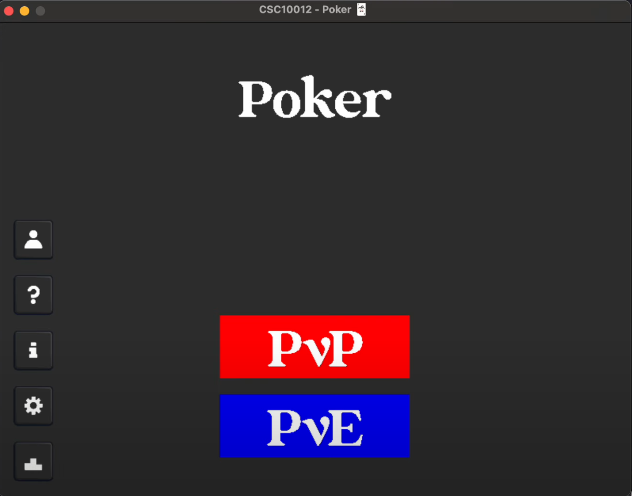
\includegraphics[width=0.7\textwidth]{figures/start_screen.png}
    \caption{Start Screen}
    \label{fig:start-screen}
\end{figure}

\hspace{1cm} The game starts with no loading screen, directly to the start screen. The start screen is simple and clean, with the game title at the top, and 5 buttons at the bottom left corner and 2 buttons at the bottom middle of the screen, each with a different function. The buttons are: 

\begin{enumerate}
    \item \textbf{User Info}: The button that has the icon of a person.
    \\ This button navigate the user to the login screen, where they can login or register a new account. You can view the login screen in \hyperref[subsec:login-screen]{Login Screen} section.
    \item \textbf{Tutorial}: The button that has the icon of a question mark.
    \\ This button navigate the user to the tutorial screen, where they can learn about the ranking of the poker hands. You can view the tutorial screen in \hyperref[subsec:tutorial-screen]{Tutorial Screen} section.
    \item \textbf{About Us}: The button that has the icon of the character "i", which stands for information.
    \\ This button navigate the user to the about us screen, where they can learn about us - the developers of this game. You can view the tutorial screen in \hyperref[subsec:about-us-screen]{About Us Screen} section.
    \item \textbf{Settings}: The button that has the icon of a gear.
    \\ This button navigate the user to the settings screen, where they can change the settings of the game, such as the background music, the sound effects, and the game mode. You can view the tutorial screen in \hyperref[subsec:settings-screen]{Settings Screen} section.
    \item \textbf{Leaderboard}: The button that has the icon of a standing podium.
    \\ This button navigate the user to the leaderboard screen, where they can view all the players and their corresponding information.
    \item \textbf{PvP}: The button that has the text "PvP" on it.
    \\ This button navigate the user to the PvP screen, based on the current game mode, the user can play either Basic Poker or Draw Poker.
    \item \textbf{PvE}: The button that has the text "PvE" on it.
    \\ This button navigate the user to the PvE screen, where the user can play Basic Poker against 5 computer players.
\end{enumerate}

\subsection{Login Screen}
\label{subsec:login-screen}

\begin{figure}[H]
    \centering
    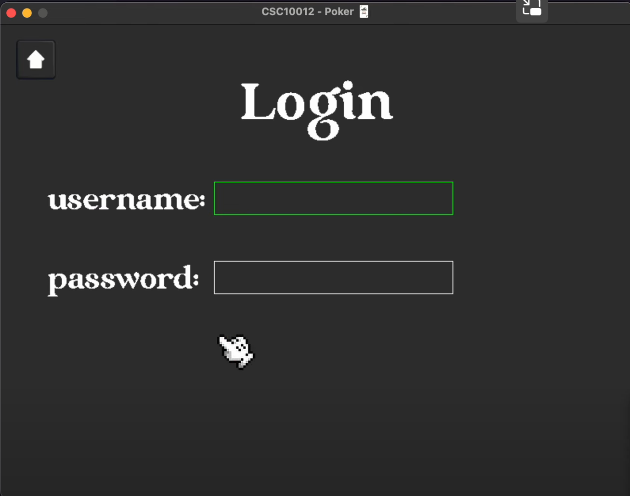
\includegraphics[width=0.7\textwidth]{figures/login_screen.png}
    \caption{Login Screen}
    \label{fig:login-screen}
\end{figure}

\hspace{1cm} The login screen is simple and clean, with the title of the screen at the top, and 2 text fields for the user to input their username and password, one downside of the screen is that user need to use \texttt{tab} key to navigate between the text fields, we have not implemented the mouse click to navigate between the text fields yet. When there is a new username, a prompt will appear to ask the user to register a new account. If the user has an existing account, they can login by inputting their username and password, then press \texttt{enter} key to login to the game. A small status message will appear at the bottom middle of the screen to inform the user about the status of their login process whether it is successful or it is an incorrect username or password. The user can navigate back to the start screen by pressing the back button at the top left corner of the screen, the button that has the icon of a house.

\vspace{0.5cm}

\hspace{1cm} You can view the demonstration video of the login screen via this \href{https://youtu.be/OA0v6xG21N4?t=165}{YouTube timestamp link}.

\subsection{Tutorial Screen}
\label{subsec:tutorial-screen}

\begin{figure}[H]
    \centering
    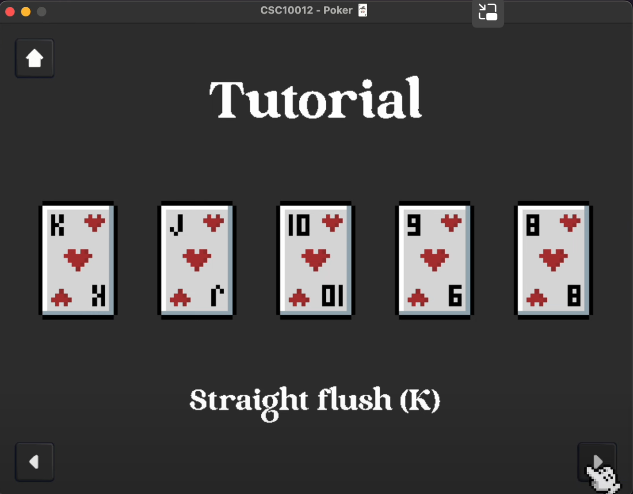
\includegraphics[width=0.7\textwidth]{figures/tutorial_screen.png}
    \caption{Tutorial Screen}
    \label{fig:tutorial-screen}
\end{figure}

\hspace{1cm} The tutorial screen is simple and intuitive, with the title of the screen at the top, and the content of the tutorial in the middle of the screen. At the bottom left corner of the screen, there is a back button that has the icon of a left arrow, which allows the user to navigate back to the previous demonstration of a hand ranking in Poker. At the bottom right corner of the screen, there is a next button that has the icon of a right arrow, which allows the user to navigate to the next demonstration of a hand ranking in Poker. The user can navigate back to the start screen by pressing the back button at the top left corner of the screen, the button that has the icon of a house. Also at the bottom middle of the screen, there is a status message that informs the user about the current demonstration of the hand they are viewing.

\vspace{0.5cm}

\hspace{1cm} You can view the demonstration video of the tutorial screen via this \href{https://youtu.be/OA0v6xG21N4?t=120}{YouTube timestamp link}.

\subsection{About Us Screen}
\label{subsec:about-us-screen}

\hspace{1cm} Unfortunately, we have not implemented the about us screen yet. The about us screen will contain information about us - the developers of this game, but we think that it is not necessary to implement this feature at the moment. We will consider implementing this feature in the future if we have time.

\subsection{Settings Screen}
\label{subsec:settings-screen}

\begin{figure}[H]
    \centering
    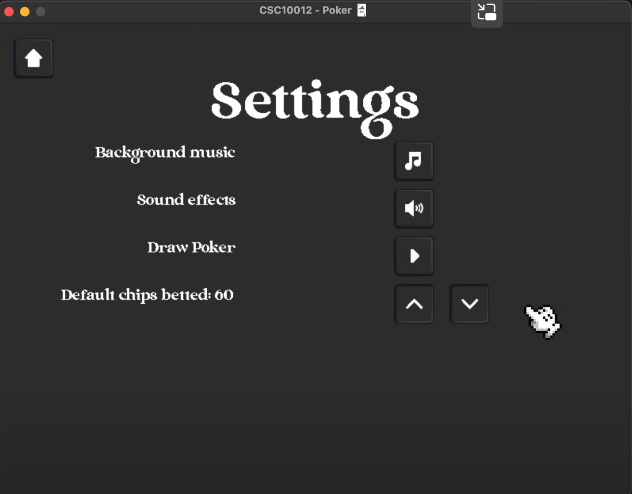
\includegraphics[width=0.7\textwidth]{figures/settings_screen.png}
    \caption{Settings Screen}
    \label{fig:settings-screen}
\end{figure}

\hspace{1cm} The settings screen is simple, with the title of the screen at the top, and 4 rows of settings that the user can change. The user can navigate back to the start screen by pressing the back button at the top left corner of the screen, the button that has the icon of a house. The 4 rows of settings are:
\begin{enumerate}
    \item \textbf{Background Music}: The first row of settings is the background music, where the user can turn on or off the background music. The user can change the background music by pressing the music note icon on the right side of the row. Notice that the background music will be turned on by default when the user starts the game. And the button will change its texture to indicate the current status of the background music.
    \item \textbf{Sound Effects}: The second row of settings is the sound effects, where the user can turn on or off the sound effects. The user can change the sound effects by pressing the sound icon on the right side of the row. And the button will change its texture to indicate the current status of the sound effects.
    \item \textbf{Game Mode}: The third row of settings is the game mode, where the user can change the game mode to either Basic Poker or Draw Poker. The user can change the game mode by pressing the right arrow icon on the right side of the row.
    \item \textbf{Default entry fee (chips)}: The fourth row of settings is the default entry fee, where the user can change the default entry fee to play the game. The user can change the default entry fee by pressing the up or down arrow icon on the right side of the row. When pressing the up arrow icon, the default entry fee will increase by 20 chips, and when pressing the down arrow icon, the default entry fee will decrease by 20 chips.
\end{enumerate}

\hspace{1cm} You can view the demonstration video of the settings screen via this \href{https://youtu.be/OA0v6xG21N4?t=144}{YouTube timestamp link}.

\subsection{Leaderboard Screen}
\label{subsec:leaderboard-screen}

\begin{figure}[H]
    \centering
    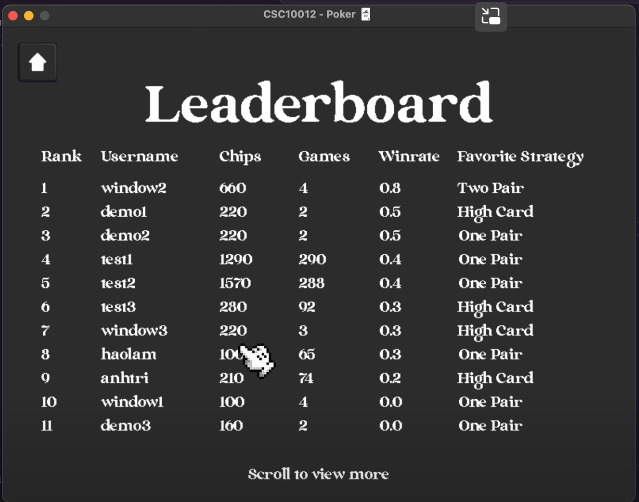
\includegraphics[width=0.7\textwidth]{figures/leaderboard_screen.png}
    \caption{Leaderboard Screen}
    \label{fig:leaderboard-screen}
\end{figure}

\hspace{1cm} In the leaderboard screen, the user can view all the registered players and their corresponding information such as their rank, username, chips, number of played games, winrate and their favorite strategy. The user can navigate back to the start screen by pressing the back button at the top left corner of the screen, the button that has the icon of a house. In this screen, if there are more than 11 players, the user can scroll through the leaderboard by using the mouse wheel.

\vspace{0.5cm}

\hspace{1cm} You can view the demonstration video of the leaderboard screen via this \href{https://youtu.be/OA0v6xG21N4?t=302}{YouTube timestamp link}.

\subsection{PvP Screen}
\label{subsec:pvp-screen}

\begin{figure}[H]
    \centering
    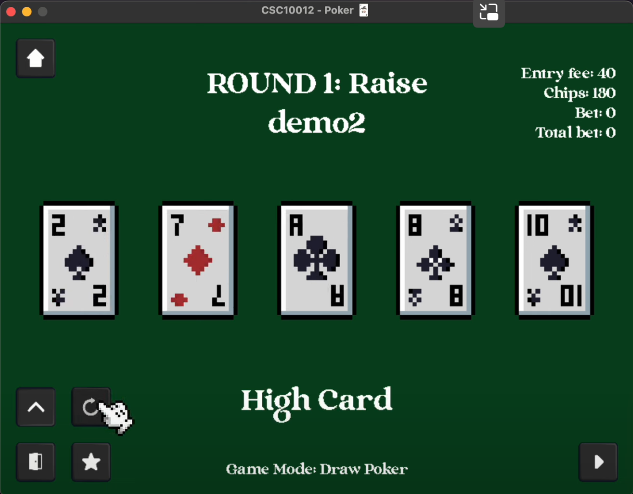
\includegraphics[width=0.7\textwidth]{figures/pvp_screen.png}
    \caption{PvP Screen}
    \label{fig:pvp-screen}
\end{figure}

\hspace{1cm} The PvP screen is one of the core features of the game, where the user can play against another player in real-time. This screen will change its render logic based on the current game mode.

\vspace{0.5cm}

\hspace{1cm} For Basic Poker game mode, the screen will display each of the player's hand and their corresponding information such as their username, chips, and their current bet. The user can click on their card to reveal the card, and click on the card again to hide the card, that's it. When all the cards facing up, a small status message will appear at the bottom middle of the screen to inform the user about the hand ranking of the player. After viewing their card, the user can click on the next button to proceed to the next player. When click that button, all of the cards of the next player will be faced down and the next player can now go to the computer and view their card. This process will repeat until all of the players have viewed their card. After that, the game will proceed to the result screen, where the winner will be announced and their card will be revealed for all the players to see.

\vspace{0.5cm}

\hspace{1cm} For Draw Poker game mode, the screen will display each of the player's hand and their corresponding information such as their username, chips, and their current bet just like the basic poker game mode. The difference here is that now the player have to deal with 4 new buttons, which are the call, raise, fold, and draw button. Here come the new mechanics of the game:
\begin{enumerate}
    \item \textbf{Call}: The call button allows the player to match the current highest bet of the game. The player can only call if they have enough chips to match the current highest bet.
    \item \textbf{Raise}: The raise button allows the player to raise their own bet, each time the player press that button, their own bet will increase by 20 chips. The player can only raise if they have enough chips to raise their own bet.
    \item \textbf{Fold}: The fold button allows the player to fold their hand, which means they will lose the current game and their bet will be taken by the winner of the game.
    \item \textbf{Draw}: The draw button allows the player to draw new cards from the deck. We have implemented the right mouse click to select the card that the player wants to draw. The player can only choose up to 3 cards to draw, and they can only draw once. After the player has drawn the card, there is nothing left they can do, they should press the next button to proceed to the next player.
\end{enumerate}

\hspace{1cm} We also handle if that button can be clicked or not in the current round of the game. It should be cleaner if we manage to also fade out the button that cannot be clicked to have a better user experience. However, we think that it is not necessary to implement this feature at the moment. We will consider implementing this feature in the future.

\vspace{0.5cm}

\hspace{1cm} Finally, you can view the demonstration video of the PvP screen Draw Poker game mode via this \href{https://youtu.be/OA0v6xG21N4?t=308}{YouTube timestamp link}.

\subsection{PvE Screen}
\label{subsec:pve-screen}

\begin{figure}[H]
    \centering
    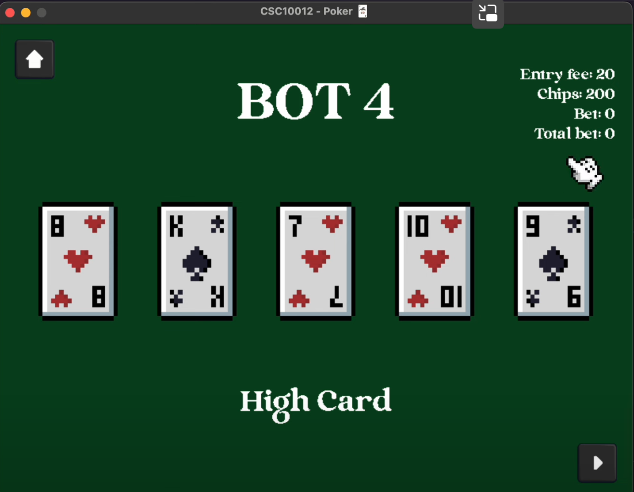
\includegraphics[width=0.7\textwidth]{figures/pve_screen.png}
    \caption{PvE Screen}
    \label{fig:pve-screen}
\end{figure}

\hspace{1cm} The PvE screen is one of the core features of the game, where the user can play against 5 computer players. This screen will not change its render logic based on the current game mode since we only support Basic Poker game mode for PvE screen. The screen will display each of the player's hand and their corresponding information such as their username, chips, and their current bet. The user can click on their card to reveal the card, and click on the card again to hide the card, that's it. When all the cards facing up, a small status message will appear at the bottom middle of the screen to inform the user about the hand ranking of the player. After viewing their card, the user can click on the next button to proceed to the next player. When click that button, all of the cards of the next player will be faced down and the next player can now go to the computer and view their card. It's just quite similar to the PvP screen, but the difference is that the user will play against 5 more bot players.

\vspace{0.5cm}

\hspace{1cm} Our bot players are quite simple, their cards will be facing up by the player click. Their information is also displayed on the screen, such as their username, chips, and their current bet. Notice that, if the player win against bots, they will not get any chips, but if they lose, they will lose the chips that they bet, since we want our game to be more challenging and closer to the real poker game where bots are quite hard to beat and have significant advantages over the player. We will consider implementing the reward system for the player if they win against bots in the future.

\vspace{0.5cm}

\hspace{1cm} Finally, you can view the demonstration video of the PvE screen via this \href{https://youtu.be/OA0v6xG21N4?t=210}{YouTube timestamp link}.

% ------------------- THE END ------------------- %

% Conclusion
\input{contents/Conclusion.tex}

% References
\pagebreak
\section{List of References}
\label{sec:references-list}

\begin{itemize}
    \item \LaTeX \space \href{https://github.com/khongsomeo/hcmus-unofficial-report-template}{template for report}.
    \item \LaTeX \space \href{https://youtu.be/4lyHIQl4VM8}{on Visual Studio Code tutorial}.
    \item \href{https://www.overleaf.com/learn/}{Overleaf documentation}.
    \item \href{https://github.com/libsdl-org/SDL/releases/tag/release-2.30.9}{SDL-2.30.9 library}
    \item \href{https://lazyfoo.net/tutorials/SDL}{SDL-2.30.9 installation tutorial}
    \item \href{https://cmake.org/download}{CMake-3.21.3 library}
    \item \href{https://aspecsgaming.itch.io/pixel-art-cursors}{Pixel Art Cursors on itch.io}.
    \item \href{https://prinbles.itch.io/analogue-buttons-pack-i}{Analogue Buttons Pack I on itch.io}.
    \item \href{https://aspecsgaming.itch.io/mini-pixel-playing-cards?download}{Mini Pixel Playing Cards on itch.io}.
    \item Discussed with classmates Nguyen Minh Duc and Hy Hue Hung.
\end{itemize}

% ------------------- THE END ------------------- %
\pagebreak
\section{List of Bugs}
\label{sec:bugs-list}

\hspace{1cm} This section lists out the bugs that were encountered during the development of the project. The bugs are categorized based on the severity of the issue and the impact it had on the project. The bugs are listed in the order of their discovery, with the most critical bugs listed first. Each bug is described in detail, including the steps to reproduce the bug, the impact it had on the project, and the solution that was implemented to fix the bug.

\begin{enumerate}
    \item \textbf{Bug: Game screen rapidly ticks} 
    \\ \textbf{Severity: Critical}, \textbf{Impact: High}, \textbf{Status: Fixed}
    \\ \textbf{Description}: This bug caused the game screen to rapidly tick, making it difficult to play the game. The bug was caused by lack of handle for the game loop, which caused the game to run at an extremely high frame rate. This resulted in the game screen rapidly ticking. \href{https://youtu.be/yJd1IkAmf3o}{Link to the video}.
    \\ \textbf{Solution}: The bug was fixed by adding a handle for the game loop, which limited the frame rate to a reasonable value such as \texttt{60} frames per second. This fixed the issue and made the game screen tick at a normal rate.
    
    \item \textbf{Bug: Leaderboard screen cannot handle large number of entries}
    \\ \textbf{Severity: Major}, \textbf{Impact: Medium}, \textbf{Status: Fixed}
    \\ \textbf{Description}: This bug not crash the game, but it caused the leaderboard screen to display incorrectly when there were a large number of entries from the csv file. The leaderboard screen can only display a limited number of entries.
    \\ \textbf{Solution}: The bug was fixed by handling mouse scroll events in the leaderboard screen. This allowed the user to scroll through the leaderboard entries using the mouse wheel. This fixed the issue and allowed the user to view all the entries in the leaderboard.
    
    \item \textbf{Bug: Betting amount not updated correctly}
    \\ \textbf{Severity: Minor}, \textbf{Impact: Low}, \textbf{Status: Fixed}
    \\ \textbf{Description}: This bug caused the betting amount to not be updated correctly when the player call or raise the bet. The betting amount was not updated correctly in the game screen, which caused confusion for the player.
    \\ \textbf{Solution}: The bug was fixed by changing some of the logic in the gameplay code.
    
    \item \textbf{Bug: Makefile not working on MacOS}
    \\ \textbf{Severity: Minor}, \textbf{Impact: Low}, \textbf{Status: Fixed}
    \\ \textbf{Description}: This bug caused the Makefile to not work on MacOS. The Makefile was not able to compile the project on MacOS due to the difference in the command line.
    \\ \textbf{Solution}: The bug was fixed by adding a conditional statement in the Makefile to check the operating system and run the appropriate command. This fixed the issue and allowed the Makefile to compile the project on MacOS.
    \item \textbf{Bug: Incorrect card images displayed}
    \\ \textbf{Severity: Minor}, \textbf{Impact: Low}, \textbf{Status: Fixed}
    
    \item \textbf{Bug: Memory leak due to too many conditional statements}
    \\ \textbf{Severity: Crucial}, \textbf{Impact: High}, \textbf{Status: Fixed}
    \\ \textbf{Description}: This bug caused a memory leak in the game due to too many conditional statements in the code, especially in the PvP screen, where we need to handle both Basic and Draw Poker mode in the same screen.
    \\ \textbf{Solution}: The bug was fixed by refactoring the code, removing unnecessary conditional statements, rename some variables, and split the code into separate functions. This fixed the issue and removed the memory leak.
    
    \item \textbf{Bug: Different password hashing on different OS}
    \\ \textbf{Severity: Major}, \textbf{Impact: High}, \textbf{Status: Not Fixed}
    \\ \textbf{Description}: This bug caused the password hashing to be different on different operating systems. The password hashing algorithm used in the project was not consistent across different operating systems, which caused the password to be hashed differently on different systems.
    \\ \textbf{Solution}: For now, the bug is not fixed. The password hashing algorithm needs to be updated to use a consistent hashing algorithm that works across different operating systems.
    
    \item \textbf{Bug: Turn off the background music does not work}
    \\ \textbf{Severity: Minor}, \textbf{Impact: Low}, \textbf{Status: Fixed}
    \\ \textbf{Description}: This bug caused the background music to not turn off when the user clicked the button to turn off the music. 
    \\ \textbf{Solution}: There is a misspelled function in the code, which caused the bug. The bug was fixed by correcting the misspell in the code.

    \item \textbf{Bug: Incorrect winner}
    \\ \textbf{Severity: Major}, \textbf{Impact: High}, \textbf{Status: Fixed}
    \\ \textbf{Description}: This bug caused the game to find the incorrect winner when the game ended. The bug was caused by incorrect logic at the early stage of the game.
    \\ \textbf{Solution}: The bug was fixed by changing the logic, adding the sorting algorithm to sort the player's hand, and finding the winner based on the sorted hand. Also archive the cards that form the rank of the player's hand for futher development.

    \item \textbf{Bug: Incorrect player id after shuffle their position}
    \\ \textbf{Severity: Major}, \textbf{Impact: High}, \textbf{Status: Fixed}
    \\ \textbf{Description}: This bug caused the player id to be incorrect after we shuffle their position. We think that shuffle the player's position will make the game more interesting and balance. However, the player id was not updated correctly after shuffling their position.
    \\ \textbf{Solution}: The bug was fixed by refactoring the code, adding one more variable which is the player's position, then use that to update the player id after shuffling their position.
\end{enumerate}

\hspace{1cm} The bugs listed above were encountered during the development of the project. Notice that, all the bugs listed above are not the only bugs that were encountered during the development process. However, these are the most time-consuming bugs that had a significant impact on the project. Finally, we manage to fix the majority of those bugs and the project is now in a stable state.

% ------------------- THE END ------------------- %

\end{document}